

\subsubsection*{Objectives}
\begin{outline}
	\1 Define:
	    \2 Gaussian Elimination
	    \2 Row echelon form
	    \2 Reduced row echelon form
	    \2 overdetermined and underdetermined systems
	    \2 Homogeneous systems
    
    \1 Reduce augmented matrix with elementary row operations
        \2 i.e., perform Gaussian elimination to reduce a matrix to echelon (or reduced echelon) form 
\end{outline}


\subsubsection*{Homework}
\textsection1.2: \#1, 6ad, 10, 16, 19 (Due 1 week)


\rule[0.01in]{\textwidth}{0.0025in}
% ------------------------------------------ % 



\begin{example}Solve the system
\[
\begin{array}{rcr}
-x_2 - x_3 + x_4 & = & 0 \\
x_1 + x_2 + x_3 + x_4 & = & 6 \\
2 x_1 + 4x_2 + x_3 - 2 x_4 & = & -1 \\
3x_1 + x_2 - 2x_3 + 2x_4 & = & 3
\end{array}
\]
\end{example}


\rule[0.01in]{\textwidth}{0.0025in}
% ------------------------------------------ % 





%
%%
%%%
%%%% SECTION:  
%%%
%%
%





Given an augmented matrix $[A | b]$ that represents a system, we perform elementary row operations to reduce to an equivalent system (ideally strictly triangular form).  The row that is being used at any step along the way is called the {\color{blue}\textbf{pivot row}}.  The first nonzero entry in the pivot row is called the {\color{blue}\textbf{pivot}} (or pivot element).

The variables corresponding to the first nonzero elements in each row of the reduced matrix are referred to as {\color{blue}\textbf{lead variables}}.  The remaining variables corresponding to the columns skipped in the process are called {\color{blue}\textbf{free variables}}.

% [Row Echelon Form]
\begin{tcolorbox}[colback=yellow!10!,colframe=gray!15!]
\begin{definition}[Row Echelon Form]
A matrix is said to be in row echelon form if
\begin{itemize}
	\item[(i)] first nonzero entry in each nonzero row is $1$
	\item[(ii)] if row $k$ is not a zero row, then number of leading zeros in row $k+1$ is greater than then number of leading zeros in row $k$.  
	\item[(iii)] all zero rows are at bottom
\end{itemize}
\end{definition}	 
\end{tcolorbox} 


\begin{example}
\[ 
 \begin{bmatrix} 
1& 1 & 1	& 2 & 5 \\
 0 & 0 & 1 & 3 & 7 \\
  0 & 0 & 0 & 0 & 1\\
    0 & 0 & 0 & 0 & 0
    \end{bmatrix} 
 \]
\end{example}














% [Reduced Row Echelon Form]
\begin{tcolorbox}[colback=yellow!10!,colframe=gray!15!]
\begin{definition}[Reduced Row Echelon Form]
A matrix is said to be in row echelon form if
\begin{itemize}
	\item[(i)] The matrix is in row echelon form
	\item[(ii)] The first nonzero entry in each row is the only nonzero entry in its column
\end{itemize}
\end{definition}	 
\end{tcolorbox} 


\begin{example}
\[ 
 \begin{bmatrix} 
1& 1 & 0	& 2 & 0 \\
 0 & 0 & 1 & 3 & 0 \\
  0 & 0 & 0 & 0 & 1\\
    0 & 0 & 0 & 0 & 0
    \end{bmatrix} 
 \]
\end{example}




\rule[0.01in]{\textwidth}{0.0025in}
% ------------------------------------------ % 




% [Gaussian Elimination]
\begin{tcolorbox}[colback=yellow!10!,colframe=gray!15!]
 \begin{definition}[Gaussian Elimination]
  process of using elementary row operations to transform augmented matrix into row echelon form (echelon = levels)
 \end{definition}
\end{tcolorbox} 













\section{Overdetermined and underdetermined Systems}

 
An {\color{blue}\textbf{overdetermined system}}  has  more equations than unknowns ($m > n$).  Typically inconsistent, but possible to have one or infinite solutions. The book gives three examples of  systems for each of the three cases (1 solution, no solution, and infinite solutions).  Here is an example of an overdetermined system.   
 


\begin{example}
$ \begin{array}{rcl}& & \\ x_1 - 3x_2 & = & 2 \\ 5x_1 - 2 x_2 & = & 7  \\ 3x_1 + x_2 &=& 1 \end{array}$
\end{example}



 

An $m \times n$  system of equations is called {\color{blue}\textbf{underdetermined}} if it has  \underline{more unknowns} than equations ($n > m$).   Typically consistent dependent (infinite number of solutions).  Possible to have no solutions, but impossible to have a unique solution.  

 



\begin{example}
$ \begin{array}{rcl}& & \\ x_1 - 3x_2  + 2 x_3 & = & 1 \\ 3x_1 + 2 x_2 - 4x_3 & = & 2 \end{array}$
\end{example}





\rule[0.01in]{\textwidth}{0.0025in}
% ------------------------------------------ % 









\section{Homogeneous Systems}
%A system is {\color{blue}\textbf{homogeneous}} if the right hand side of the system consists of all zeros.  

A {\color{blue}\textbf{homogeneous linear system}} of $m$ equations in $n$ unknowns is then a system of the form: 
\[ 
\begin{cases} 
a_{11} x_1 + a_{12} x_2 + a_{13} x_3 + \dots + a_{1n} x_n = 0\\
 a_{21} x_1 + a_{22} x_2 + a_{23} x_3 + \dots + a_{2n} x_n = 0\\
a_{31} x_1 + a_{32} x_2 + a_{33} x_3 + \dots + a_{3n} x_n = 0\\

\hfill \vdots \hfill \vdots \hfill \vdots \\

a_{m1} x_1 + a_{m2} x_2 + a_{m3} x_3 + \dots + a_{mn} x_n = 0
\end{cases} .
 \]


 

\begin{example}
$ \begin{array}{rcl}& & \\ x_1 - 3x_2 & = & 0 \\ 5x_1 - 2 x_2 & = & 0 \end{array}$
\end{example}






%\[  {\bf b} = \begin{bmatrix}
%	0 \\ 0 \\ \vdots \\ 0
%	\end{bmatrix}
% \]



\textbf{Fact}: Homogeneous systems are always \textit{consistent} (i.e., the trivial solution). 

\begin{theorem}
An $m \times n$ homogeneous system of linear equations has a nontrivial solution if $n > m$ (i.e., underdetermined system).  
\end{theorem}


% The letter ${\bf v}$ was used to emphasize \textbf{v}ector, but other common letters used include ${\bf a, b, c, u, w, x, y, z}$.  For instance,  a three-dimensional vector could be represented as follows (note the use of both square and rounded brackets): 

 



 
\textbf{One solution}
 \[ 
 \begin{bmatrix}[cccc|c] 
1& 0 & 0	& 0 & x \\
 0 & 1 & 0 & 0 & x \\
  0 & 0 & 1 & 0 &  x \\
    0 & 0 & 0 & 1 & x
    \end{bmatrix} 
 \]



\textbf{Infinite solutions} (free variable)
 \[ 
 \begin{bmatrix}[cccc|c] 
1& 0 & x	& 0 & x \\
 0 & 1 & 1 & 0 & x \\
  0 & 0 & 0 & 1 &  x \\
    0 & 0 & 0 & 0 & 0
    \end{bmatrix} 
 \]


 
\textbf{No solutions} (Nonsense equation)
 \[ 
 \begin{bmatrix}[cccc|c] 
1& 0 & 0	& x & x \\
 0 & 1 & 0 & x & x \\
  0 & 0 & 1 & 0 &  x \\
    0 & 0 & 0 & 0 & x
    \end{bmatrix} 
 \]








\rule[0.01in]{\textwidth}{0.0025in}
% ------------------------------------------ % 



\begin{example}
Suppose a city consists of sets of one-way streets.  The average hourly volume of traffic entering and leaving each intersection is given by the diagram.  Determine the amount of traffic between each intersection (See Figure below).
        \begin{figure}[htbp] %  figure placement: here, top, bottom, or page
           \centering
           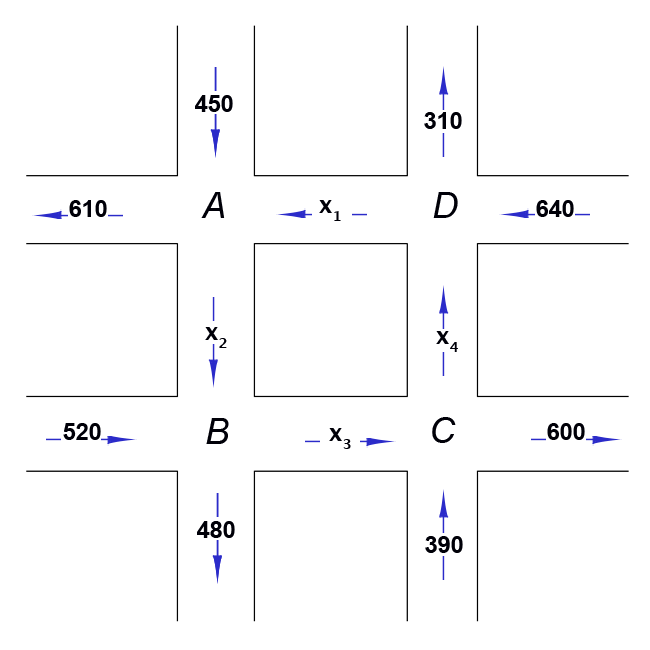
\includegraphics[width=4in]{figures/trafficflow.png} 
           \caption{Average Hourly Volume of Traffic in City Center}
           \label{fig:trafficflow}
        \end{figure}
        



{\bf Solution:}

$ \begin{cases} A: 450 + x_1  = 610 + x_2 \\  B: 520 + x_2 = 480 + x_3 \\ C: 390 + x_3 = 600 + x_4 \\ D: 640 + x_4 = 310 + x_1  \end{cases} $
 $\rightarrow$
$ \begin{cases} A:  x_1 - x_2  = 160 \\  B: x_2 - x_3 = -40  \\ C: x_3 - x_4 = 210 \\ D:  x_4 - x_1 = -330  \end{cases} $
 $\rightarrow$
$  \begin{bmatrix} [cccc|c]
1 & -1 & 0 & 0 & 160 \\
0 & 1 & -1 & 0 & -40 \\
0 & 0 & 1 & -1 & 210 \\
-1 & 0 & 0 & 1 & -330 
  \end{bmatrix} $

$\rightarrow$
$  \begin{bmatrix} [cccc|c]
1 & -1 & 0 & 0 & 160 \\
0 & 1 & -1 & 0 & -40 \\
0 & 0 & 1 & -1 & 210 \\
0 & -1 & 0 & 1 & -170 
  \end{bmatrix} $
$\rightarrow$
$  \begin{bmatrix} [cccc|c]
1 & 0 & -1 & 0 & 120 \\
0 & 1 & -1 & 0 & -40 \\
0 & 0 & 1 & -1 & 210 \\
0 & 0 & -1 & 1 & -210 
 \end{bmatrix} $
 $\rightarrow$
$  \begin{bmatrix} [cccc|c]
1 & 0 & 0 & -1 & 330 \\
0 & 1 & 0 & -1 & 170 \\
0 & 0 & 1 & -1 & 210 \\
0 & 0 & 0 & 0 & 0 
 \end{bmatrix} $

$\rightarrow$
$ \begin{cases}  x_1 -x_4 = 330  \\  x_2 - x_4 = 170  \\  x_3 -x_4  = 210 \\  x_4 = \alpha  \end{cases} $
$\rightarrow$
$\begin{bmatrix} [c]
330 + \alpha \\ 
170 + \alpha \\
210 + \alpha \\
\alpha 
 \end{bmatrix} $ 

\end{example}

















\rule[0.01in]{\textwidth}{0.0025in}
% ------------------------------------------ % 









%\subsubsection*{Next time...}
%Section 1.3:  Matrix Arithmetic 












\subsection*{Additional Examples}

These can be done by hand or with GeoGebra.  

\begin{outline}[enumerate]

	

\1 (Chapter 1.1).  Solve each of the systems represented by the augmented matrix.
 
% -------- 
\2 $  \begin{bmatrix} [cc|c]
3& 2 & 8 \\
 1 & 5 & 7  \end{bmatrix} $  

\bf{Solution:}
$  \begin{bmatrix} [cc|c]
3& 2 & 8 \\
 1 & 5 & 7  \end{bmatrix} $
 $\rightarrow$
$  \begin{bmatrix} [cc|c]
 3 & 2 & 8 \\
 0 & \frac{13}{3} & \frac{13}{3}  \end{bmatrix} $
 $ \rightarrow $
$ \begin{cases} 3x_1 + 2x_2 = 8 \\  \frac{13}{3}x_2 = \frac{13}{3}   \end{cases} $
$\rightarrow$
$ \begin{bmatrix} [c]
 2 \\
 1 \\
 \end{bmatrix} $ 


\item $  \begin{bmatrix} [ccc|c]
1& -2 & 1 & 3 \\
2 & 3 & -4 &  0
  \end{bmatrix} $ 
  
\bf{Solution:}

$  \begin{bmatrix} [ccc|c]
1& -2 & 1 & 3 \\
2 & 3 & -4 &  0
  \end{bmatrix} $
  $\rightarrow$
$  \begin{bmatrix} [ccc|c]
1& -2 & 1 & 3 \\
0 & 7 & -6 &  -6
  \end{bmatrix} $
  $\rightarrow$
$  \begin{bmatrix} [ccc|c]
1& -2 & 1 & 3 \\
0 & 1 & -\frac{6}{7} &  -\frac{6}{7}
  \end{bmatrix} $
  $\rightarrow$
$  \begin{bmatrix} [ccc|c]
1 & 0 & -\frac{5}{7} & \frac{9}{7} \\
0 & 1 & -\frac{6}{7} &  -\frac{6}{7}
  \end{bmatrix} $  
  
  $\rightarrow$ 
$ \begin{cases} x_1 - \frac{5}{7}x_3 = \frac{9}{7} \\  x_2 - \frac{6}{7}x_3 = -\frac{6}{7}   \end{cases} $  
 $\rightarrow$ 
$ \begin{cases} x_1 = \frac{9}{7} + \frac{5}{7}x_3 \\  x_2 = -\frac{6}{7} + \frac{6}{7}x_3 \end{cases} $
$\rightarrow$
$\begin{bmatrix} [c]
\frac{9}{7} + \frac{5}{7}\alpha \\
-\frac{6}{7} + \frac{6}{7}\alpha \\
\alpha 
\end{bmatrix} $ 
  




\2  $  \begin{bmatrix} [ccc|c]
2 & 1 & 4 & -1 \\
4 & -2 & 3 &  4 \\
5 & 2 & 6 &  -1
  \end{bmatrix} $  
  
\bf{Solution:}
  
$  \begin{bmatrix} [ccc|c]
2 & 1 & 4 & -1 \\
4 & -2 & 3 &  4 \\
5 & 2 & 6 &  -1
  \end{bmatrix} $
  $\rightarrow$
$  \begin{bmatrix} [ccc|c]
2 & 1 & 4 & -1 \\
0 & -4 & -5 &  6 \\
0 & -\frac{1}{2} & -4 & \frac{3}{2}
  \end{bmatrix} $  
  $\rightarrow$
$  \begin{bmatrix} [ccc|c]
2 & 1 & 4 & -1 \\
0 & -4 & -5 &  6 \\
0 & 0 & -\frac{27}{8} & \frac{3}{4}
  \end{bmatrix} $    
  $\rightarrow$
$ \begin{cases} 2x_1 + x_2 + 4x_3 = -1 \\  -4x_2 - 5x_3 = 6 \\ -\frac{27}{8}x_3 = \frac{3}{4}   \end{cases} $

$\rightarrow$
$\begin{bmatrix} [c]
\frac{5}{9} \\ 
-\frac{11}{9}\\ 
-\frac{2}{9}
\end{bmatrix} $ 







\2  $  \begin{bmatrix} [cccc|c]
2 & 1 & 4 & -1 & 4 \\
3 & 1 & -5 &  6  & 5\\
1 & 1 & 2 &  4 & 8 \\
5 & 1 & 3 &  -2 & 7
  \end{bmatrix} $
  

\bf{Solution:}  
  
$  \begin{bmatrix} [cccc|c]
2 & 1 & 4 & -1 & 4 \\
3 & 1 & -5 &  6  & 5\\
1 & 1 & 2 &  4 & 8 \\
5 & 1 & 3 &  -2 & 7
  \end{bmatrix} $
  $\rightarrow$
$  \begin{bmatrix} [cccc|c]
2 & 1 & 4 & -1 & 4 \\
0 & -\frac{1}{2} & -11 & \frac{15}{2}  & -1\\
0 & \frac{1}{2} & 0 & \frac{9}{2} & 6 \\
0 & -\frac{3}{2} & -7 & \frac{1}{2} & -3
  \end{bmatrix} $
  $\rightarrow$
$  \begin{bmatrix} [cccc|c]
2 & 1 & 4 & -1 & 4 \\
0 & -\frac{1}{2} & -11 & \frac{15}{2} & -1\\
0 & 0 & -11 & 12 & 5 \\
0 & 0 & 26 & -22 & 0
  \end{bmatrix} $
  
  $\rightarrow$
$  \begin{bmatrix} [cccc|c]
2 & 1 & 4 & -1 & 4 \\
0 & -\frac{1}{2} & -11 & \frac{15}{2} & -1\\
0 & 0 & -11 & 12 & 5 \\
0 & 0 & 0 & \frac{70}{11} & \frac{130}{11}
  \end{bmatrix} $
  $\rightarrow$
$ \begin{cases} 2x_1 + x_2 + 4x_3 - x_4 = 4 \\  \frac{1}{2}x_2 - 11x_3 + \frac{15}{2}x_4 = -1 \\ -11x_3 + 12x_4 = 5 \\ \frac{70}{11}x_4 = \frac{130}{11}   \end{cases} $
  $\rightarrow$
  $\begin{bmatrix} [c]
  \frac{15}{7} \\
  -\frac{33}{7} \\
  \frac{11}{7} \\
  \frac{13}{7} \\
  \end{bmatrix} $ 
 
 

	
 

\end{outline}


 

